\documentclass[oneside]{amsart}
\usepackage[12pt]{extsizes}
\usepackage{graphicx,amssymb,mathtools,mathrsfs,geometry,xcolor}
\renewcommand{\theequation}{\alph{equation}}
\newcommand{\cfbox}[2]{%
    \colorlet{currentcolor}{.}%
    {\color{#1}%
    \fboxrule=2pt
    \fbox{\color{currentcolor}#2}}%
}
\title{Proposition 4.1}
\begin{document}
\begin{center}
    \fbox{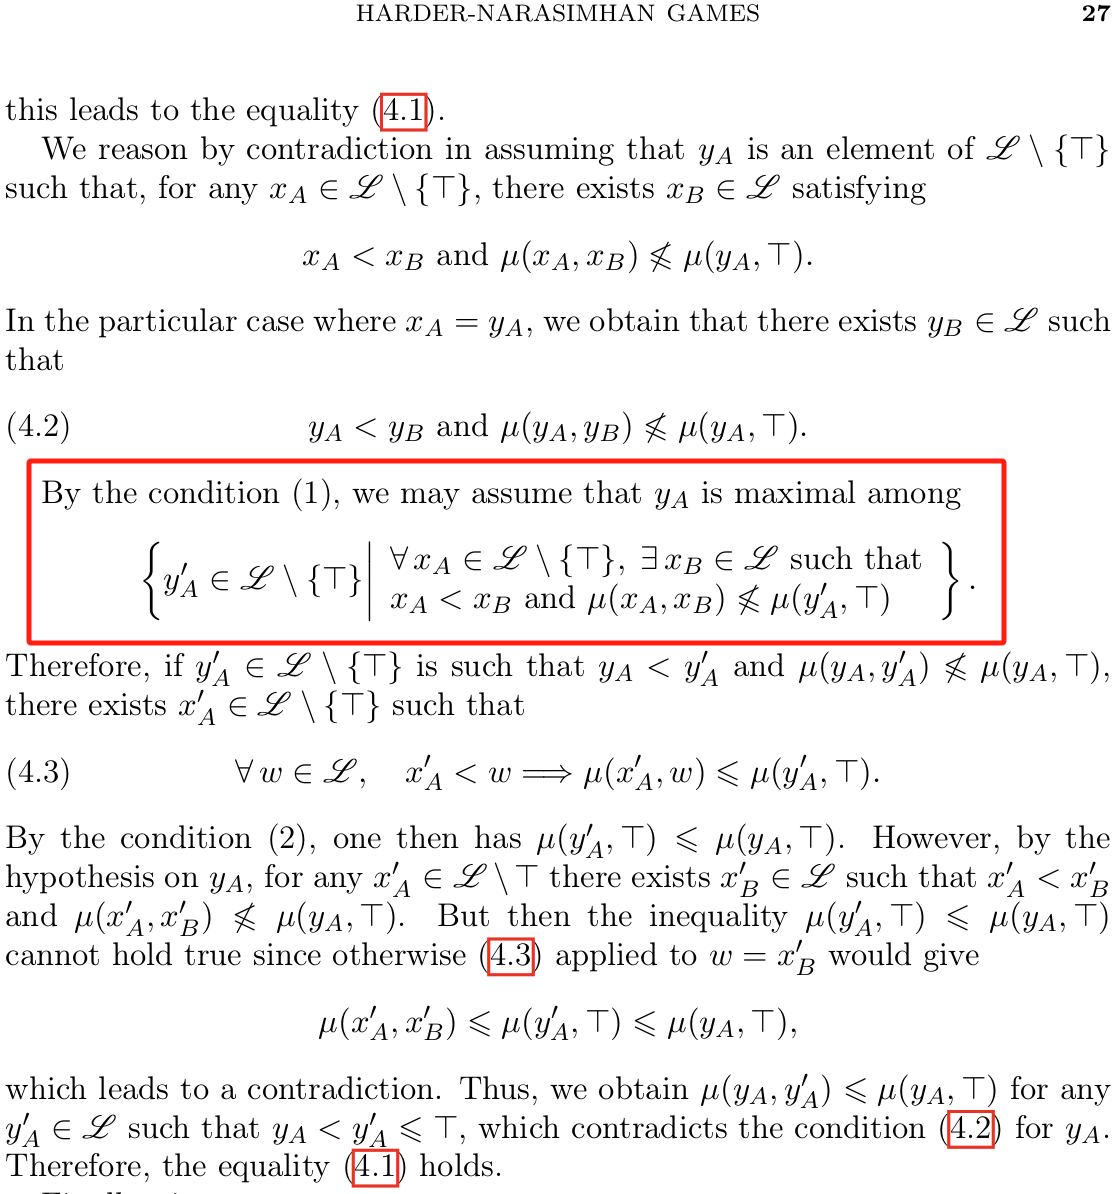
\includegraphics[width=\textwidth]{p4d1.png}}
\end{center}
\clearpage
I'm not quite understand how the \cfbox{red}{argument} works. If we set

$$\mathcal{S}\coloneqq \left\{y_A'\in \mathscr{L}\backslash \{\top\}\middle\vert\substack{\forall x_A\in \mathscr{L}\backslash\{\top\}, \ \exists x_B\in\mathscr{L}\ \text{such that}\\x_A<x_B \text{ and }\mu(x_A,x_B)\not\leq \mu(y_A',\top)}\right\},$$
then the whole screenshot aims to show that $\mathcal{S}$ is empty by contradiction.

So after using contradiction, $\mathcal{S}$ is not empty with certain $y_A\in \mathcal{S}$. The \cfbox{red}{argument} is telling us that there exists (at least) a maximal element $y_{A,\max}$ in $\mathcal{S}$, then we just take the place of $y_A$ by $y_{A,\max}$. I believe this is what ``we may assume that $y_A$ is maximal'' means. The \cfbox{red}{argument} suggests us to show the existence of $y_{A,\max}$ by the Condition (1). I have two different unsuccessful attempts towards this goal as follows:
\begin{enumerate}
    \item If $y_{A,\max}$ does not exist, then we can recursively define a strictly increasing sequence $x_0=y_A<x_1<\cdots<x_n<\cdots$ in $\mathcal{S}$. By the Condition (1), there exists $N\in\mathbb{N}$ such that
\begin{equation}
    \mu(x_N,x_{N+1})\leq\mu(x_N,\top).
\end{equation}
Then I don't know how to continue. By the definition of $\mathcal{S}$, there exists $x_B'\in\mathscr{L}$ such that $x_N<x_B'$ and $\mu(x_N,x_B')\not\leq \mu(x_N,\top)$. However, this does not seem to contradict (a), as $x_B'$ is not necessarily equals to $x_{N+1}$.
\item Start with $x_0=y_A$, by (4.2) there exists $x_1\in\mathscr{L}$ such that $x_0<x_1$ and $\mu(x_0,x_1)\not\leq \mu(x_0,\top)$. If $x_1$ can be chosen in $\mathcal{S}$, then we can apply (4.2) on $x_1$ to get $x_2\in\mathscr{L}$ such that $x_1<x_2$ and $\mu(x_1,x_2)\not\leq \mu(x_1,\top)$. This process can not goes on forever, otherwise we get a strictly increasing sequence $x_0<x_1<\cdots$ in $\mathcal{S}$ such that $\mu(x_n,x_{n+1})\not\leq \mu(x_n,\top)$ for all $n\in\mathbb{N}$, which contradicts Condition (1). Therefore there exists $k\in\mathbb{N}$ such that $x_k\in\mathcal{S}$ and for every $y\in \mathcal{S}$, we have
\begin{align*}
    &\neg (x_k < y \land \mu(x_k,y)\not\leq \mu(x_k,\top))\\
    =&(x_k\not<y)\lor (x_k<y \land \mu(x_k,y)\leq \mu(x_k,\top)).
\end{align*}
What we want is $x_k\not< y$ (for every $y\in \mathcal{S}$), but I don't know how to rule out the case $x_k<y \land \mu(x_k,y)\leq \mu(x_k,\top)$. (4.2) is not applicable here, as we have another constraint that $y\color{red}\in\mathcal{S}$.
\end{enumerate}



\end{document}